% questions.tex —— 2007 年·全国大纲卷Ⅰ·理科 · 题目内容片段（无答案）
% 由 tools/generate_projects.py 依来源总账自 2007/2007_数学真题_全国1理_试题.md 生成，勿手改（改源 MD 后重跑）


\gkpart{数学}

\begin{gktip}
\textbf{来源说明}：本题面依据固定源 PDF 两页 A3 题面逐题转录，原卷印刷页码 359–360。固定源不附答案，答案和解析均由本库独立复算。

\textbf{图形说明}：第 7、19 题的原卷图形关系重绘为 TikZ/PGFPlots 矢量图。图形标记所指的 PNG 不随仓库保存。
\end{gktip}

\gkpart{一、选择题}

\begin{question}
\gkti{1}$\alpha$ 是第四象限角，$\tan\alpha=-\dfrac5{12}$，则 $\sin\alpha=$\mbox{（　　）}

（A）$\dfrac15$\quad（B）$-\dfrac15$\quad（C）$\dfrac5{13}$\quad（D）$-\dfrac5{13}$

\end{question}
\begin{question}
\gkti{2}设 $a$ 是实数，且 $\dfrac{a}{1+i}+\dfrac{1+i}{2}$ 是实数，则 $a=$\mbox{（　　）}

（A）$\dfrac12$\quad（B）$1$\quad（C）$\dfrac32$\quad（D）$2$

\end{question}
\begin{question}
\gkti{3}已知向量 $\boldsymbol a=(-5,6)$，$\boldsymbol b=(6,5)$，则 $\boldsymbol a$ 与 $\boldsymbol b$\mbox{（　　）}

（A）垂直\quad（B）不垂直也不平行\quad（C）平行且同向\quad（D）平行且反向

\end{question}
\begin{question}
\gkti{4}已知双曲线的离心率为 $2$，焦点是 $(-4,0),(4,0)$，则双曲线方程为\mbox{（　　）}

（A）$\dfrac{x^2}{4}-\dfrac{y^2}{12}=1$\quad（B）$\dfrac{x^2}{12}-\dfrac{y^2}{4}=1$\quad（C）$\dfrac{x^2}{10}-\dfrac{y^2}{6}=1$\quad（D）$\dfrac{x^2}{6}-\dfrac{y^2}{10}=1$

\end{question}
\begin{question}
\gkti{5}设 $a,b\in\mathbb R$，集合 $\{1,a+b,a\}=\left\{0,\dfrac ba,b\right\}$，则 $b-a=$\mbox{（　　）}

（A）$1$\quad（B）$-1$\quad（C）$2$\quad（D）$-2$

\end{question}
\begin{question}
\gkti{6}下面给出的四个点中，到直线 $x-y+1=0$ 的距离为 $\dfrac{\sqrt2}{2}$，且位于不等式组

\nopagebreak[4]
\[
\begin{cases}
x+y-1<0,\\
x-y+1>0
\end{cases}
\]

表示的平面区域内的点是\mbox{（　　）}

（A）$(1,1)$\quad（B）$(-1,1)$\quad（C）$(-1,-1)$\quad（D）$(1,-1)$

\Needspace{0.4\textheight}
\end{question}
\begin{question}
\gkti{7}如图，正四棱柱 $ABCD-A_1B_1C_1D_1$ 中，$AA_1=2AB$，则异面直线 $A_1B$ 与 $AD_1$ 所成角的余弦值为\mbox{（　　）}
\nopagebreak[4]
\begin{center}% 2007 年全国大纲卷Ⅰ理科第 7 题：正四棱柱
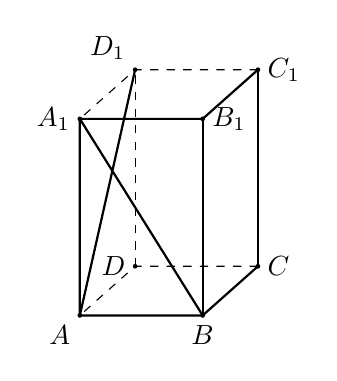
\begin{tikzpicture}[>=stealth,scale=0.78]
  \coordinate (A) at (0,0); \coordinate (B) at (2.0,0);
  \coordinate (C) at (2.9,0.8); \coordinate (D) at (0.9,0.8);
  \coordinate (A1) at (0,3.2); \coordinate (B1) at (2,3.2);
  \coordinate (C1) at (2.9,4.0); \coordinate (D1) at (0.9,4.0);
  \draw[thick] (A)--(B)--(C); \draw[dashed] (C)--(D)--(A);
  \draw[thick] (A)--(A1)--(B1)--(C1);
  \draw[dashed] (C1)--(D1)--(A1);
  \draw[thick] (B)--(B1) (C)--(C1);
  \draw[dashed] (D)--(D1);
  \draw[thick] (A1)--(B) (A)--(D1);
  \fill (A) circle (1.1pt) node[below left] {$A$};
  \fill (B) circle (1.1pt) node[below] {$B$};
  \fill (C) circle (1.1pt) node[right] {$C$};
  \fill (D) circle (1.1pt) node[left] {$D$};
  \fill (A1) circle (1.1pt) node[left] {$A_1$};
  \fill (B1) circle (1.1pt) node[right] {$B_1$};
  \fill (C1) circle (1.1pt) node[right] {$C_1$};
  \fill (D1) circle (1.1pt) node[above left] {$D_1$};
\end{tikzpicture}
\end{center}
\nopagebreak[4]
（A）$\dfrac15$\quad（B）$\dfrac25$\quad（C）$\dfrac35$\quad（D）$\dfrac45$

\end{question}
\begin{question}
\gkti{8}设 $a>1$，函数 $f(x)=\log_a x$ 在区间 $[a,2a]$ 上的最大值与最小值之差为 $\dfrac12$，则 $a=$\mbox{（　　）}

（A）$\sqrt2$\quad（B）$2$\quad（C）$2\sqrt2$\quad（D）$4$

\end{question}
\begin{question}
\gkti{9}$f(x),g(x)$ 是定义在 $\mathbb R$ 上的函数，$h(x)=f(x)+g(x)$，则“$f(x),g(x)$ 均为偶函数”是“$h(x)$ 为偶函数”的\mbox{（　　）}

（A）充要条件\quad（B）充分而不必要的条件\quad（C）必要而不充分的条件\quad（D）既不充分也不必要的条件

\end{question}
\begin{question}
\gkti{10}在 $\left(x^2-\dfrac1x\right)^n$ 的展开式中，常数项为 $15$，则 $n=$\mbox{（　　）}

（A）$3$\quad（B）$4$\quad（C）$5$\quad（D）$6$

\end{question}
\begin{question}
\gkti{11}抛物线 $y^2=4x$ 的焦点为 $F$，准线为 $l$，经过 $F$ 且斜率为 $\sqrt3$ 的直线与抛物线在 $x$ 轴上方的部分相交于点 $A$，$AK\perp l$，垂足为 $K$，且 $\triangle AKF$ 的面积是\mbox{（　　）}

（A）$4$\quad（B）$3\sqrt3$\quad（C）$4\sqrt3$\quad（D）$8$

\end{question}
\begin{question}
\gkti{12}函数 $f(x)=\cos^2x-2\cos^2\dfrac x2$ 的一个单调增区间是\mbox{（　　）}

（A）$\left(\dfrac\pi3,\dfrac{2\pi}3\right)$\quad（B）$\left(\dfrac\pi6,\dfrac\pi2\right)$\quad（C）$\left(0,\dfrac\pi3\right)$\quad（D）$\left(-\dfrac\pi6,\dfrac\pi6\right)$

\end{question}
\gkpart{二、填空题}

\begin{question}
\gkti{13}从班委会 $5$ 名成员中选出 $3$ 名，分别担任班级学习委员、文娱委员与体育委员，其中甲、乙二人不能担任文娱委员，则不同的选法共有\gkblank{}种。（用数字作答）

\end{question}
\begin{question}
\gkti{14}函数 $y=f(x)$ 的图象与函数 $y=\log_3x\ (x>0)$ 的图象关于直线 $y=x$ 对称，则 $f(x)=$\gkblank{}。

\end{question}
\begin{question}
\gkti{15}等比数列 $\{a_n\}$ 的前 $n$ 项和 $S_n$，已知 $S_1,2S_2,3S_3$ 成等差数列，则 $\{a_n\}$ 的公比为\gkblank{}。

\end{question}
\begin{question}
\gkti{16}一个等腰直角三角形的三个顶点分别在正三棱柱的三条侧棱上。已知正三棱柱的底面边长为 $2$，则该三角形的斜边长为\gkblank{}。

\end{question}
\gkpart{三、解答题}

\begin{question}
\gkti{17}设锐角三角形 $ABC$ 的内角 $A,B,C$ 的对边分别为 $a,b,c$，$a=2b\sin A$。

（1） 求 $B$ 的大小；

（2） 求 $\cos A+\sin C$ 的取值范围。

\end{question}
\begin{question}
\gkti{18}某商场经销某商品，根据以往资料统计，顾客采用的付款期为随机变量 $\xi$ 的分布列为

\begin{center}
\begin{tabular}{lrrrrr}
\toprule
$\xi$ & $1$ & $2$ & $3$ & $4$ & $5$ \\
\midrule
$P$ & $0.4$ & $0.2$ & $0.2$ & $0.1$ & $0.1$ \\
\bottomrule
\end{tabular}
\end{center}

商场经销一件该商品，采用 $1$ 期付款，基利润为 $200$ 元；分 $2$ 期或 $3$ 期付款，基利润为 $250$ 元；分 $4$ 期或 $5$ 期付款，其利润为 $300$ 元。$\eta$ 表示经销一件该商品的利润。

（1） 求事件 $A$：“购买该商品的 $3$ 位顾客中，至少有 $1$ 位采用 $1$ 期付款”的概率 $P(A)$；

（2） 求 $\eta$ 的分布列及期望 $E\eta$。

\Needspace{0.4\textheight}
\end{question}
\begin{question}
\gkti{19}四棱锥 $S-ABCD$ 中，底面 $ABCD$ 为平行四边形，侧面 $SBC\perp$ 底面 $ABCD$。已知 $\angle ABC=45^\circ$，$AB=2$，$BC=2\sqrt2$，$SA=SB=\sqrt3$。
\nopagebreak[4]
\begin{center}% 2007 年全国大纲卷Ⅰ理科第 19 题：四棱锥
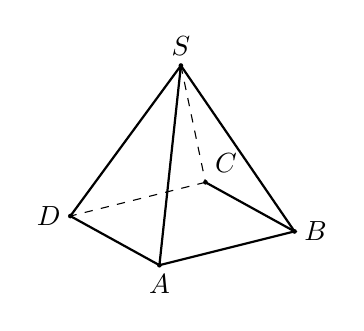
\begin{tikzpicture}[>=stealth,scale=0.78]
  \coordinate (A) at (1.8,0); \coordinate (B) at (4.0,0.55);
  \coordinate (C) at (2.55,1.35); \coordinate (D) at (0.35,0.8);
  \coordinate (S) at (2.15,3.25);
  \draw[thick] (A)--(B)--(C); \draw[dashed] (C)--(D); \draw[thick] (D)--(A);
  \draw[thick] (S)--(A) (S)--(B) (S)--(D);
  \draw[dashed] (S)--(C);
  \fill (S) circle (1.1pt) node[above] {$S$};
  \fill (A) circle (1.1pt) node[below] {$A$};
  \fill (B) circle (1.1pt) node[right] {$B$};
  \fill (C) circle (1.1pt) node[above right] {$C$};
  \fill (D) circle (1.1pt) node[left] {$D$};
\end{tikzpicture}
\end{center}
\nopagebreak[4]
（1） 证明：$SA\perp BC$；

（2） 求直线 $SD$ 与平面 $SAB$ 所成角的大小。

\end{question}
\begin{question}
\gkti{20}设函数 $f(x)=e^x-e^{-x}$。

（1） 证明：$f(x)$ 的导数 $f'(x)\geqslant2$；

（2） 若对所有 $x\geqslant0$ 都有 $f(x)\geqslant ax$，求 $a$ 的取值范围。

\end{question}
\begin{question}
\gkti{21}已知椭圆 $\dfrac{x^2}{3}+\dfrac{y^2}{2}=1$ 的左、右焦点分别为 $F_1,F_2$，过 $F_1$ 的直线交椭圆于 $B,D$ 两点，过 $F_2$ 的直线交椭圆于 $A,C$ 两点，且 $AC\perp BD$，垂足为 $P$。

（1） 设 $P$ 点的坐标为 $(x_0,y_0)$，证明：$\dfrac{x_0^2}{3}+\dfrac{y_0^2}{2}<1$；

（2） 求四边形 $ABCD$ 的面积的最小值。

\end{question}
\begin{question}
\gkti{22}已知数列 $\{a_n\}$ 中 $a_1=2$，$a_{n+1}=(\sqrt2-1)(a_n+2)$，$n=1,2,3,\ldots$。

（1） 求 $\{a_n\}$ 的通项公式；

（2） 若数列 $\{b_n\}$ 中 $b_1=2$，$b_{n+1}=\dfrac{3b_n+4}{2b_n+3}$，$n=1,2,3,\ldots$，证明：$b_n<b_{n+1}$，其中 $n$ 为正整数。

\end{question}